\documentclass{article}
\usepackage[UTF8]{ctex}
\usepackage{tikz}

\begin{document}

    \begin{center}
    \vspace{50pt}
    {
        \zihao{1}
        \bf
        武汉大学计算机学院 \\
        本科生课程设计报告
    }
    \end{center}

    \begin{center}
    \vspace{50pt}
    {
        \zihao{2}
        \bf
        RISC-V CPU 设计
    }
    \end{center}

    \begin{center}
    \vspace{50pt}
    {
        \large{}
        \begin{tabular}{ll}
            专业名称:& 计算机科学与技术 \\
            课程名称:& 计算机系统综合设计 \\
            指导老师:& 蔡朝晖\  副教授 \\
                      & 陈伟清\  高级实验师 \\
            学生学号:& 2020302191485 \\
            学生姓名:& 朱\ 卓\ 远 \\
        \end{tabular}
    }
    \end{center}

    \vspace{100pt}

    \begin{center}
        {
            \zihao{3}
            二〇二二年七月
        }
    \end{center}

    \newpage{}
    \begin{center}
    {
        \zihao{2}
        \bf
        郑\ 重\ 声\ 明
    }
    \end{center}
    \vspace{20pt}
    {
        \normalsize{}
        \par{}
        本人呈交的实验报告,是在指导老师的指导下,独立进行实验工作所取得的成果,所有数据、图片资料真实可靠。尽我所知,除文中已经注明引用的内容外,本实验报告不包含他人享有著作权的内容。对本实验报告做出贡献的其他个人和集体,均已在文中以明确的方式标明。本实验报告的知识产权归属于培养单位。
    }
    \vspace{20pt}
    {
        \normalsize{}
        \newline{}
        本人签名:\ \ \ \ \ \ \ \ \ \ \ \ \ \ \ \ \ \ \ \ \ \ \ \ \ \ \ \ 
        日期:
    }

    \newpage{}
    \LARGE{}
    \begin{center}
        \bf
        \Large{}
        摘要
    \end{center}
    \vspace{10pt}
    \normalsize{}
    \par{}
        计算机系统课程设计的目的在于,通过设计支持RISCV32基础指令集的CPU,熟练掌握RISCV32基础指令集,深入理解单周期和流水线CPU的数据通路和控制通路。
    \par{}
        实验内容主要包括:单周期CPU、五级流水线CPU和双发射五级流水线CPU。
    \vspace{10pt}
    \newline{}
    {\bf 关键词:}单周期、流水线、双发射

    \newpage{}

    \begin{center}
    \zihao{-2}
    {\bf 目 \ \ \ \ 录}
    \end{center}

    {
        \zihao{-4}
        \renewcommand{\contentsname}{}
        \tableofcontents
    }
    \newpage{}
    \section{引言}
        \subsection{实验目的}
        \par{}
        通过设计支持RISCV32基础指令集的CPU,深化对RISCV架构的理解,深入理解CPU的数据通路和控制通路,培养计算机系统能力。
        \subsection{国内外研究现状}
        \par{}
        RISC-V指令集架构师一个机遇RISC原则开发的开源指令集架构,由加州大学伯克利分校的Krste Asanovic教授领导设计,Patterson教授也参与了这一项目。与大多数指令集相比,RISC-V指令集可以自由的用于任何目的,允许任何人设计、制造和销售RISC-V芯片和软件而不必支付给任何公司专利费。\cite{ref2}
        \par{}
        香山高性能开源RISC-V处理器项目是我国RISC-V研究的标志性项目,由中国科学院计算技术研究所牵头发起。该项目研发出目前国际上性能最高的开源高性能RISC-V处理器核“香山”。香山处理器目前已经进行到第三版的研发阶段。第一版雁栖湖架构已于2021年7月投片,在28nm工艺节点下达到1.3GHz频率,第二版南湖架构已于2022年3月完成RTL代码冻结,目标于14nm工艺节点下频率达到2GHz。香山处理器核使用Chisel语言开发,在开发过程中同时搭建了DiffTest框架、创制了NEMU模拟器等开源基础工具,为教学和科学研究做出了卓越的贡献。\cite{ref3}
    \newpage{}
    \section{实验环境介绍}
        \subsection{Verilog HDL}
        Verilog是一种用于描述、设计电子系统(特别是)数字电路的硬件描述语言,主要用于集成电路设计。Verilog能够在多种抽象级别对数字逻辑系统进行描述,同时能够用于逻辑仿真和综合,从而便于在FPGA上实现硬件电路。\cite{ref4}
        \subsection{Icarus Verilog}
        Icarus Verilog是Verilog硬件描述语言的实现工具,提供了Verilog编译器,并通过一个虚拟机对设计进行仿真。\cite{ref5}
        \subsection{GTKWave}
        GTKWave是一种波形查看工具,其支持vcd、lx2等格式的波形文件打开。
        \subsection{Xilinx ISE}
        Xilinx ISE是一款由Xilinx开发的用于合成和分析HDL设计的软件工具,开发者可以使用Xilinx ISE综合自己的设计、执行时序分析、检查RTL图、仿真不同激励下的设计的响应,并使用编程器配置目标设备。\cite{ref6}
        \subsection{SWORD}
        SWORD,全称Simple While Organic aRc Design,是一种计算机系统能力培养方法。其内容涵盖了从数字逻辑硬件设计,到指令集架构设计与扩展,并延伸到编译器设计,甚至涵盖了操作系统设计与实现,及基于上述一切内容的计算机系统集成设计与应用。\cite{ref7}
        \subsection{objdump和as}
        objdump和as是由我使用C++语言编写的反汇编和汇编代码。objdump用于将16进制指令比特转换为RISC-V汇编代码,而as则用于将RISC-V汇编代码转换为16进制指令比特。使用时只需要用g++或clang编译器编译生成可执行文件即可。

    \newpage{}
    \begin{figure}[ht]
        \centering
        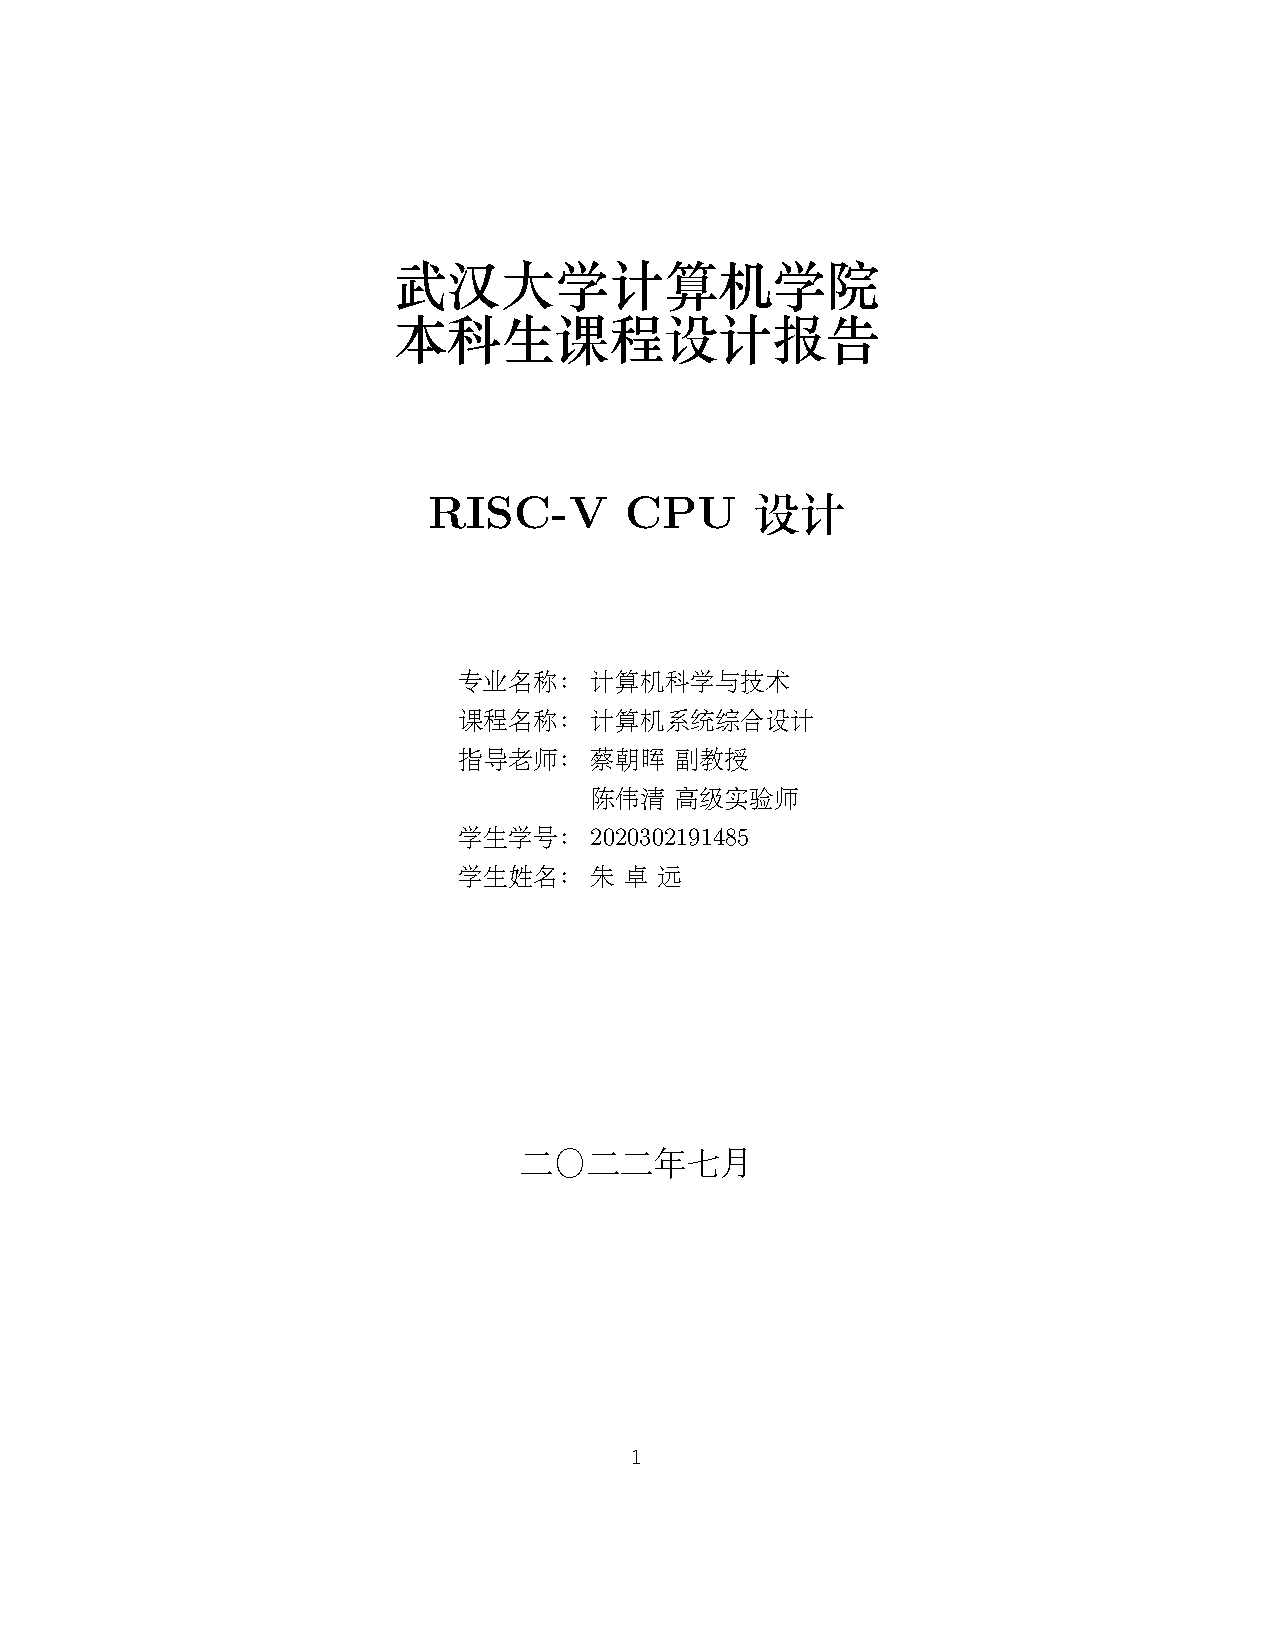
\includegraphics[width=1\textwidth]{a.jpg}
        \caption{单周期与五级流水线设计}
    \end{figure}
    \section{单周期CPU设计}    
        \subsection{pcReg}
            \par{}
            pcReg用于更新下一个周期的PC寄存器的值。在RISCV32基础指令集中,有3种不同的PC寄存器更新方式,即PC+4、PC+imm、rs1+imm。其中PC+imm的控制方式也分为两种,第一种是有条件跳转,由beq、bne等比较指令的比较结果决定,第二种是无条件跳转。
            \par{}
            我对之的处理方式较为简单,即将pc\_src控制信号扩充为2位。低位0表示选择+4,1表示选择+imm,高位0表示选择pc,1表示选择rs1。当处理有条件跳转时,只需要将低位信号与zero的值相与,即可完成筛选过程。
            \par{}
            选择过程采用组合逻辑,代码如下:

            \begin{verbatim}
assign npc = (pc_src[1] ? reg_data1 : pc) 
          + ((pc_src[0] & zero) ? imm : 4);
            \end{verbatim}

        \subsection{controlUnit}
            \par{}
            controlUnit主要由两部分构成,第一步是译码,第二步是生成相应的控制信号。
            \par{}
            译码过程非常暴力,我将语句分为r\_type、ri\_type、load\_type、s\_type、sb\_type、jalr\_ins、jal\_ins、auipc\_ins、lui\_ins九大类,然后分别以他们的opcode、func3、func7作为特征,判断是否为对应的指令信号。
            \par{}
            生成控制信号的过程较为简单,对使该信号为1的指令信号执行或运算。值得一提的是我对alu\_op和mem\_op的处理。
            \par{}
            针对alu\_op,如果执行的是r型和ri型指令,则直接使用其func3,如果是其余指令,则将alu\_op置为3'b000。这样做的目的是,当执行其他类型的指令时,ALU的结果默认输出为输入ALU的数之和,极大的简化了相应的信号处理。
            \par{}
            针对mem\_op,如果执行的是load型或s型指令,则直接使用其func3,如果是其余指令,则将mem\_op置为3'b000。这样做的目的是,在执行其他指令时,从mem中返回的结果必定为32'dxxxxxxxx,倘若执行过程中出现以32'dxxxxxxxx数据作为写回数据的情况,可以精准的定位和调试。


        \subsection{immGen}
            \par{}
            immGen单元的作用是生成立即数,其受controlUnit单元中的imm\_op信号控制。我对不同的立即数处理方式进行了编号,以方便进行处理,具体编号情况以及对应的imm拓展方式如下:

            \begin{verbatim}
assign imm_op = (
    {3{r_type}} & 3'd0 | //0
    {3{ri_type | load_type | jalr_ins}} & 3'd1 | //[31:20] to [11:0]
    {3{s_type}} & 3'd2 | //[31:25], [11:7] to [11:5], [4:0]
    {3{sb_type}} & 3'd3 | //[31:25], [11:7] to [12|10:5], [4:1|11]
    {3{jal_ins}} & 3'd4 | //[31:12] to [20|10:1|11|19:12]
    {3{auipc_ins | lui_ins}} & 3'd5 //[31:12] to [31:12]
    );
            \end{verbatim}

        \subsection{regFile}
            \par{}
            regFile单元是寄存器堆,读寄存器是组合逻辑,写寄存器是时序逻辑。唯一需要注意的是,不可以对x0进行写操作。

        \subsection{compareUnit}
            \par{}
            compareUnit单元执行比较运算,其操作由controlUnit产生的compu\_op控制。其产生的zero信号控制有条件跳转的结果。

        \subsection{ALUSource}
            \par{}
            九种不同指令的ALU操作结果如下表所示

            \begin{center}
                \begin{tabular}{|c|c|}
                \hline
                r\_type & $rd = rs1 \ op \ rs2$ \\
                ri\_type & $rd = rs1 \ op \  imm$ \\
                load\_type & $rd = rs1 + imm$ \\
                s\_type & $rd = rs1 + imm$ \\
                sb\_type & $rd = rs1 \ op \  rs2$ \\
                jalr\_ins & $rd = pc + 4$ \\
                jal\_ins & $rd = pc + 4$ \\
                auipc\_ins & $rd = pc + imm$ \\
                lui\_ins & $rd = 0 + imm$ \\
                \hline
                \end{tabular}
            \end{center}
            
            \par{}
            观察上表可知,alu\_data1操作数来源只有3种:rs1、pc、0,alu\_data2操作数来源也只有3种:rs2、imm、4。因此我们只需要使用两个多路选择器即可选择两种操作数。他们分别由alu\_src1和alu\_src2信号控制。信号与对应结果如下表所示: 

            \begin{center}
                \begin{tabular}{|c|c|}
                \hline
                alu\_src1 & alu\_data1 \\
                \hline
                0 & rs1 \\
                1 & pc \\
                2 & 0 \\
                \hline
                alu\_src2 & alu\_data2 \\
                \hline
                0 & rs2 \\
                1 & imm \\
                2 & 4 \\
                \hline
                \end{tabular}
            \end{center}

        \subsection{ALU}
            \par{}
            ALU单元的实现比较暴力,我使用组合逻辑电路来实现。首先将每一种运算的结果计算出来,之后使用一个多路选择器根据其alu\_op进行选择。

        \subsection{cpu2Mem}
            \par{}
            cpu2Mem单元用于CPU和数据内存进行交互。
            \par{}
            如果当前指令的类型为store类型,则依照mem\_op调整wea的值。否则统一将mem\_op置为4'b0000,具体代码如下:
            
            \begin{verbatim}
assign wea = mem_write ? 
(
    ({4{mem_op == `sb_func3}} & 4'b0001) |
    ({4{mem_op == `sh_func3}} & 4'b0011) |
    ({4{mem_op == `sw_func3}} & 4'b1111)
) :
    4'b0000
;
            \end{verbatim}

            \par{}
            如果当前指令为load类型,则依照mem\_op对取得的32位数据进行处理。具体代码如下:

            \begin{verbatim}
assign data_from_mem_out = 
    {32{(mem_op == `lb_func3)}} 
        & {{24{data_from_mem_in[7]}}, data_from_mem_in[7:0]} |
    {32{(mem_op == `lh_func3)}} 
        & {{16{data_from_mem_in[15]}}, data_from_mem_in[15:0]} |
    {32{(mem_op == `lw_func3)}} 
        & data_from_mem_in |
    {32{(mem_op == `lbu_func3)}} 
        & {24'b0, data_from_mem_in[7:0]} |
    {32{(mem_op == `lhu_func3)}} 
        & {16'b0, data_from_mem_in[15:0]};
            \end{verbatim}

        \subsection{wbMux}
            \par{}
            wbMux是一个二路选择器,依据mem\_2\_reg信号选择写回寄存器的数据的来源,默认情况下为ALU的计算结果。

    \newpage{}
    \section{五级流水线CPU设计}
        \subsection{流水线寄存器}
        \par{}
        在第3章对单周期CPU的讨论中,除了pc寄存器和寄存器堆外,其余的逻辑单元都为组合逻辑单元。这表明在同一时钟周期内,整个电路完成了除pc更新和寄存器堆写回之外的所有任务。而以上两种任务,则需要在下一周期上升沿到来时完成。
        \par{}
        由此可以得出将整个电路划分为五级流水线的方法。我使用四个流水线寄存器来将整个电路划分为五个阶段。当每个阶段完成后,将其准备好的信号提供给下一个流水线级。在时钟上升沿来临时,这些信号被写入下一级流水线寄存器中。
        \par{}
        因此流水线寄存器具有两个作用:第一,为本级流水线提供所需要的所有信号;第二,阻隔前一级流水线信号向本级传输。
        \par{}
        值得注意的是,在单周期CPU中,寄存器堆最终更新是在下一个周期上升沿到来之际。因此完全执行完成一条指令需要两个周期。在五级流水线CPU中同理,一条指令真正完成寄存器的写回工作是在其第6个周期进行的,这对于前递任务产生了重要的影响。

        \subsection{流水线级数的划分}
        \begin{center}
            \begin{tabular}{|c|c|}
            \hline
                IF & pcReg、controlUnit、immGen \\
                ID & compareUnit、regFile、jmpMux \\
                EX & ALUSource、ALU \\
                MEM & cpu2Mem \\
                WB & wbMux \\
            \hline
            \end{tabular}
        \end{center}

        \subsection{控制冒险}

        \begin{center}
            \begin{tabular}{|c|c|}
            \hline
                type & nextpc \\
            \hline
                r\_type & pc = pc + 4 \\
                ri\_type & pc = pc + 4 \\
                load\_type & pc = pc + 4 \\
                s\_type & pc = pc + 4 \\
                sb\_type & pc = pc + 4/imm \\
                jalr\_ins & pc = rs1 + imm \\
                jal\_ins & pc = pc + imm \\
                auipc\_ins & pc = pc + 4 \\
                lui\_ins & pc = pc + 4 \\
            \hline
            \end{tabular}
        \end{center}
        
        \par{}
        上表所示为不同指令的nextpc情况。我选择如下策略进行处理:
        \par{}
        首先将controlUnit和immGen单元前提至IF阶段,以实现半分支预测,减少周期浪费。针对跳转指令,默认其必定跳转。因此除jalr\_ins和sb\_type类型之外的指令都能正确得到其nextpc。
        \par{}
        针对sb\_type类型指令,我分离出比较单元compareUnit,并将之放置在ID阶段。因此如果分支预测错误,只会造成一个周期的浪费。
        \par{}
        针对jalr\_ins类型指令,因为rs1的值只有在ID阶段才能从寄存器堆中取出,因此势必会造成一个周期的浪费。
        \par{}
        因此,针对以上两种情况,我额外添件了IF\_flush信号,当该信号为真时,清空在上升沿清空IF\_ID寄存器,并且将正确的nextpc值赋给pc寄存器。
        \par{}
        flush信号产生代码如下:
        \begin{verbatim}
assign IF_flush = is_jalr_ins | is_sb_type & ~zero;
        \end{verbatim}
        \par{}
        nextpc的更新如下:
        \begin{verbatim}
npc = IF_flush ? jmp_data : (pc_reg + (pc_src ? imm : 32'd4));
        \end{verbatim}
        \par{}
        我使用jmpMux单元来选择flush后更新给pc寄存器的值。只有当指令为有条件跳转指令且比较的结果为假时才会选择pc + 4,否则一律选择rs1 + imm。具体代码如下:
        \begin{verbatim}
wire jmp_src = is_sb_type & ~zero;
assign jmp_data = jmp_src ? (pc + 32'd4) : (rs1 + imm);
        \end{verbatim}

        \subsection{数据冒险}
        \par{}
        在帕特森和亨尼斯的《计算机组成与设计·硬件/软件接口》{\cite{ref1}}中,对于数据冒险的解决讨论如下:
        \par{}
        以如下指令序列为例:
        \begin{verbatim}
        sub x2, x1, x3      (1)
        and x12, x2, x5     (2)
        or x13, x6, x2      (3)
        add x14, x2, x2     (4)
        sd x15, 100(x2)     (5)
        \end{verbatim}
        \par{}
        当(2)指令执行到EX阶段时,(1)指令执行到MEM阶段,此时它已经得到结果,因此可以前递到ID\_EX寄存器之后,通过一个多路选择器选择成为alu的操作数;
        \par{}
        当(3)指令执行到EX阶段时,(1)指令执行到WB阶段,此时它已经得到结果,因此可以前递到ID\_EX寄存器之后,通过一个多路选择器选择成为alu的操作数;
        \par{}
        当(4)指令执行到EX阶段时,课本上的描述如下:因为寄存器堆前半个周期写,后半个周期读,在(1)指令处于WB阶段时,它实际上已经在前半个周期将答案写进寄存器堆中,因此后半个周期读出的寄存器堆的答案为写回后的答案。因此当(4)指令执行到EX阶段时,rs1和rs2的值是准确的,无需前递。
        \par{}
        当(5)指令执行到EX阶段时,寄存器堆已经更新,rs1和rs2的值是准确的,无需前递。
        \newline{}
        \par{}
        但是,根据前文讨论,我们并不能做到寄存器堆前半个周期写,后半个周期读,因为寄存器堆的写信号是受CPU的clk控制的。与之相反,寄存器堆的写入是在WB阶段的下一个周期的上升沿,此时读出的rs1和rs2的值已经进入EX阶段参与运算。因此,如果选择这种方式,WB写回的信号将被忽略,造成错误。
        \par{}
        针对这种情况,我采取如下措施:
        \par{}
        将前递的位置由流水线寄存器后改为流水线寄存器之前。即在EX、MEM、WB三个阶段一完成运算,立即前递到ID\_EX寄存器前的多路选择器中,对之进行筛选。筛选后的结果,在上升沿写入流水线寄存器中,参与运算。
        \par{}
        这样做的另一优势在于,其有效利用了流水线寄存器封锁对应流水线阶段的信号作用。如果采用课本上的这种前递方式,当存在除法运算或者使用dcache且发生dcache miss时,如果当前阶段的信号是由前递产生的,那么在某一流水线阶段长时间停顿的时候,可能发出前递信号的指令已经写回,前递信号消失,导致答案错误,因此称课本上的这种前递方式为不稳定前递。而采取前递至寄存器堆前的方法,能利用寄存器的功能有效的锁住写回的前递信号,确保答案的正确,因此称之为稳定前递。
        \newline{}
        \par{}
        针对这种前递方式考虑数据冒险的情况,其处理情况如下表所示:
        \begin{center}
            \begin{tabular}{|c|c|c|c|}
            \hline
                数据冒险情况 & 运算结束阶段 & 前递/停顿 & 数据来源 \\
            \hline
                ID\_rs == EX\_rd & ex\_finish & 前递 & alu\_data \\ 
                ID\_rs == EX\_rd & mem\_finish & 停顿 & / \\ 
                ID\_rs == MEM\_rd & ex\_finish & 前递 & alu\_data \\
                ID\_rs == MEM\_rd & mem\_inish & 前递 & mem\_data \\
                ID\_rs == WB\_rd & no matter & 前递 & wb\_data \\
            \hline
            \end{tabular}
        \end{center}
        \par{}
        采用如下方式产生停顿:使用ID\_stall信号。当上升沿来临时,如果ID\_stall信号为真,不让pcReg和IF\_ID寄存器发生变化,清空ID\_EX寄存器。
        \par{}
        接下来考虑优先级问题。首先是多个冒险之间的优先级,易得EX > MEM > WB。其次是ID\_stall和IF\_flush信号之间的优先级,因为比较的结果和跳转的结果都收到rs2的影响,因此当两者发生冲突时,应该先stall,得到正确的结果,再判断是否flush,即ID\_stall > IF\_flush。
        \par{}
        此外,考虑一种特殊情况。当前ID阶段的指令为store类型,EX阶段的指令为load类型,但是load前递的对象为rs2时,因为rs2的值在MEM阶段才会使用,因此这种情况无需停顿,可以通过将MEM阶段访存结果前递到EX\_MEM寄存器之前来更新rs2的值。    
        \newline{}
        \begin{figure}[ht]
            \centering
            \includegraphics[width=1\textwidth]{b.jpg}
            \caption{五级流水线前递示意图}
        \end{figure}
        \par{}
        整体代码如下:
        \begin{verbatim}
//IF_ID_ForwardingUnit
assign rs1_data_out = 
 (IF_ID_rs1 != 0 && IF_ID_rs1 == ID_EX_rd && 
  ex_ex_finish) ? 
    ex_alu_data :
 (IF_ID_rs1 != 0 && IF_ID_rs1 == EX_MEM_rd && 
  mem_ex_finish) ? 
    mem_alu_data :
 (IF_ID_rs1 != 0 && IF_ID_rs1 == EX_MEM_rd && 
  mem_mem_finish) ? 
    mem_data :
 (IF_ID_rs1 != 0 && IF_ID_rs1 == MEM_WB_rd) ? 
    rd_data :
    rs1_data_in;

assign rs2_data_out = 
 (IF_ID_rs2 != 0 && IF_ID_rs2 == ID_EX_rd && 
  ex_ex_finish) ? 
    ex_alu_data :
 (IF_ID_rs2 != 0 && IF_ID_rs2 == EX_MEM_rd && 
  mem_ex_finish) ? 
    mem_alu_data :
 (IF_ID_rs2 != 0 && IF_ID_rs2 == EX_MEM_rd && 
  mem_mem_finish) ? 
    mem_data :
 (IF_ID_rs2 != 0 && IF_ID_rs2 == MEM_WB_rd) ? 
    rd_data :
    rs2_data_in;

//ID_EX_ForwardingUnit
assign rs2_data_fresh =
 (ID_EX_rs2 != 0 && ID_EX_rs2 == EX_MEM_rd && 
  mem_ex_finish) ? 
    alu_data :
 (ID_EX_rs2 != 0 && ID_EX_rs2 == EX_MEM_rd && 
  mem_mem_finish) ? 
    mem_data :
 (ID_EX_rs2 != 0 && ID_EX_rs2 == MEM_WB_rd) ? 
    rd_data :
    rs2_data_in;

//stall    
assign ID_stall = 
 (ex_mem_finish && 
  ID_EX_rd != 0 && (ID_EX_rd == IF_ID_rs1 | ID_EX_rd == IF_ID_rs2) && 
 ~IF_ID_is_s_type) | 
 (ex_mem_finish && 
  ID_EX_rd != 0 && (ID_EX_rd == IF_ID_rs1) && 
  IF_ID_is_s_type);
        \end{verbatim}

    \newpage{}
    \section{双发射五级流水线CPU设计}
        \subsection{双发射调度}
        \begin{center}
        \par{\bf 无冒险情况下两条指令是否可以发射}
        \par{}
        \begin{tabular}{|c|c|c|c|c|c|c|c|c|c|}
            \hline
                / & r & ri & load & s & sb & jalr & jal & auipc & lui \\
            \hline
                r & v & v & v & v & x & x & x & v & v \\
            \hline
                ri & v & v & v & v & x & x & x & v & v \\
            \hline
                load & v & v & v & x & x & x & x & v & v \\
            \hline
                s & v & v & x & x & x & x & x & v & v \\
            \hline
                sb & v & v & v & v & x & x & x & v & v \\
            \hline
                jalr & v & v & v & v & x & x & x & v & v \\
            \hline
                jal & v & v & v & v & x & x & x & v & v \\
            \hline
                auipc & v & v & v & v & x & x & x & v & v \\
            \hline
                lui & v & v & v & v & x & x & x & v & v \\
            \hline
        \end{tabular}

        \vspace{20pt}
        \par{\bf 有冒险情况下两条指令是否可以同时发射}
        \par{}
        \begin{tabular}{|c|c|c|c|c|c|c|c|c|c|}
            \hline
                / & r & ri & load & s & sb & jalr & jal & auipc & lui \\
            \hline
                r & x & x & x & v & x & x & x & x & x \\
            \hline
                ri & x & x & x & v & x & x & x & x & x \\
            \hline
                load & x & x & x & x & x & x & x & x & x \\
            \hline
                s(rs1) & x & x & x & x & x & x & x & x & x \\
            \hline
                s(rs2) & v & v & x & x & x & x & x & v & v \\
            \hline
                sb & x & x & x & v & x & x & x & x & x \\
            \hline
                jalr & x & x & x & v & x & x & x & x & x \\
            \hline
                jal & v & v & v & v & x & x & x & v & v \\
            \hline
                auipc & v & v & v & v & x & x & x & v & v \\
            \hline
                lui & v & v & v & v & x & x & x & v & v \\
            \hline
        \end{tabular}
        \end{center}
        \par{}
        依据上述两表,新增一个twoIssueDecide单元判断是否可以同时发射两条指令,如果可以将two\_issue信号置为1,反之置为0。
        
        \subsection{新增数据和控制通路}
        将除pc寄存器,寄存器堆,控制冒险处理单元和数据冒险处理单元之外的原有的功能单元复制一份,得到一条新的通路。本实验中存在一个可以改进的地方,即存在两条从cpu到dm的数据通路。在本实验中,直接选择bram作为内存,因此我设置了一个双端口ram,可以从两条数据通路分别操作。但是如果使用dcache,则不能如此随意的进行操作,否则会导致cache状态机混乱和axi总线发生结构冒险。正确的做法应该是新添加一个组合单元,对相关信号进行选择,保证每一次只有一条数据通路访问dcache和axi总线。这留待进一步的修改和优化。

        \subsection{寄存器堆的修改}
        将寄存器堆修改为双口读和双口写。当两条指令同时写寄存器堆时,如果两者写的寄存器一致,则将第二条指令的值赋给寄存器。

        \subsection{pc寄存器和控制冒险单元的修改}
        \par{}
        在上文所示的两表中,我严格控制了每一次仅有最多一条分支指令发射,而且当该分支指令在通路1发射时,通路2不发射指令,因此控制冒险的出现情况其实与单发射相同。唯一需要变化的是需要选择出分支指令所在的通路,这通过判断ID阶段的two\_issue信号就能直接解决。
        \par{}
        对于pc寄存器的修改也与发射情况相关。如果只发射一条指令,那么下一条指令的pc值与单发射情况相同,如果发射两条指令,下一条指令的pc值与单发射情况下pc+4的情况相同。

        \subsection{数据冒险单元的修改}
        \par{}
        上文已经提及,对于单发射情况下的数据冒险处理方式有两种,前递和停顿。双发射对于数据冒险单元的处理稍复杂一些,因为需要在两条数据通路之间通信。
        \par{}
        先考虑停顿的情况。当两条通路中的任意一条需要停顿的时候,正确的做法应该是同时将这两条通路均停顿。如果只停发生数据冒险的通路,则会造成乱序到达的后果。在顺序流水线中,这种结果是不可接受的。如果要使CPU支持这种停顿方式,有一易一难两种方法。较易的方法是,顺序发射指令、乱序执行指令、顺序提交指令。这是一种较为简单的乱序处理方式,唯一需要的是在WB阶段添加一个提交单元,以满足顺序提交的要求。较难的方式是在ID阶段设置保留站,使用动态调度算法,乱序发射指令、乱序执行指令、顺序提交指令。这样能减少停顿的次数,充分利用流水线级。前者多用于常见的RISC处理器,而后者在Intel处理器中屡见不鲜。但是这两种方法在出现dcache miss时,都需要将两条通路停顿。因为当出现dcache miss时,动辄造成20个以上的周期浪费。等待dcache的结果过程中,如果另一条通路正在执行指令,那么最坏情况下,提交单元内可能存在20条以上的指令等待提交。这将造成巨大的硬件资源损耗。
        \par{}
        再考虑前递的情况。为满足两条指令之间的交互,前递单元的优先级需要做适当的修改。其原则可以概括为八个字:前优于后,下优于上。即在不同流水线级的前递优先级为:EX > MEM > WB,在相同流水线级的两条指令之间的前递优先级,通路2的优先级高于通路1。这是因为在单发射流水线中,通路2指令肯定在通路1指令之后执行。因此,通路2得到的结果要比通路1得到的结果更新,优先级也更高。
        \begin{figure}[ht]
            \centering
            \includegraphics[width=1\textwidth]{c.jpg}
            \caption{双发射五级流水线前递示意图}
        \end{figure}

        \subsection{CPU接口的修改与总体电路的调整}
        \par{}
        将取指令接口和读写数据接口都改为双接口,在总体电路中添加一个ROM直接与CPU相连,将单口RAM改为真双端口RAM,便于双口进行读写。

    \newpage{}
    \section{测试及结果分析}
        \subsection{仿真测试}
        \par{}
        仿真测试代码如下:
        \begin{verbatim}
ori x5, x0, 564
lui x6, 1
or x5, x5, x6
lui x6, 624485
addi x7, x5, 837
addi x8, x6, -1024
xori x9, x5, 1980
sltiu x3, x7, 52
sltiu x4, x5, -1
andi x18, x9, 1893
slti x20, x6, 291
sub x19, x6, x5
xor x21, x20, x6
add x22, x21, x20
add x22, x22, x5
sub x23, x22, x6
or x25, x23, x22
and x26, x23, x22
slt x27, x25, x26
sltu x28, x25, x26
addi x3, x3, 4
sll x27, x26, x3
srl x28, x25, x3
sra x29, x25, x3
slli x27, x19, 16
srli x28, x19, 4
srai x29, x19, 4
addi x3, x0, 768
addi x5, x0, 255
sw x19, 0(x3)
sw x21, 4(x3)
sw x23, 8(x3)
sh x26, 4(x3)
sh x19, 10(x3)
sb x5, 7(x3)
sb x5, 9(x3)
sb x5, 8(x3)
lw x5, 0(x3)
sw x5, 12(x3)
lh x7, 2(x3)
sw x7, 16(x3)
lhu x7, 2(x3)
sw x7, 20(x3)
lb x8, 3(x3)
sw x8, 24(x3)
lbu x8, 3(x3)
sw x8, 28(x3)
lbu x8, 1(x3)
sw x8, 32(x3)
sw x0, 0(x3)
and x9, x0, x9
bne x5, x7, 8
addi x9, x9, 1
bge x5, x7, 8
addi x9, x9, 4
bgeu x5, x7, 8
addi x9, x9, 2
blt x5, x7, 8
addi x9, x9, 7
bltu x5, x7, 0
addi x9, x9, 8
beq x7, x8, 8
addi x9, x9, 10
sw x9, 0(x3)
ori x30, x0, 1397
lw x10, 0(x3)
jal x1, 16
addi x10, x10, 5
sw x10, 0(x3)
beq x10, x30, 48
ori x10, x10, 1360
sw x10, 0(x3)
jalr x0, x1, 0
jal x1, 32
add x0, x0, x0
add x0, x0, x0
add x0, x0, x0
add x0, x0, x0
add x0, x0, x0
add x0, x0, x0
add x0, x0, x0
lui x4, 1048575
srai x4, x4, 12
add x5, x4, x4
add x5, x5, x5
add x5, x5, x5
add x5, x5, x5
add x5, x5, x5
add x5, x5, x5
ori x20, x0, 63
add x5, x5, x5
add x5, x5, x5
add x5, x5, x5
add x5, x5, x5
add x5, x5, x5
add x5, x5, x5
add x5, x5, x5
add x5, x5, x5
add x5, x5, x5
add x5, x5, x5
add x5, x5, x5
add x5, x5, x5
add x5, x5, x5
add x5, x5, x5
add x5, x5, x5
add x5, x5, x5
add x5, x5, x5
add x5, x5, x5
add x5, x5, x5
add x5, x5, x5
add x6, x5, x5
add x5, x6, x6
add x7, x5, x5
add x13, x7, x7
add x8, x13, x13
sltu x9, x0, x4
add x14, x9, x9
add x14, x14, x14
add x10, x4, x4
sw x6, 4(x5)
lw x25, 0(x5)
add x25, x25, x25
add x25, x25, x25
sw x25, 0(x5)
add x19, x19, x9
sw x19, 0(x7)
lw x13, 20(x0)
lw x25, 0(x5)
add x25, x25, x25
add x25, x25, x25
sw x25, 0(x5)
lw x25, 0(x5)
and x11, x25, x8
add x13, x13, x9
beq x13, x0, 96
lw x25, 0(x5)
add x18, x14, x14
add x22, x18, x18
add x18, x18, x22
and x11, x25, x18
beq x11, x0, 24
beq x11, x18, 44
add x18, x14, x14
beq x11, x18, 48
sw x19, 0(x7)
jal x1, -72
beq x10, x4, 8
jal x1, 12
or x10, x4, x0
add x10, x10, x10
sw x10, 0(x7)
jal x1, -96
lw x19, 96(x17)
sw x19, 0(x7)
jal x1, -108
lw x19, 32(x17)
sw x19, 0(x7)
jal x1, -120
lw x13, 20(x0)
add x10, x10, x10
or x10, x10, x9
add x17, x17, x14
and x17, x17, x20
add x19, x19, x9
beq x19, x4, 8
jal x1, 12
add x19, x0, x14
add x19, x19, x9
lw x25, 0(x5)
add x11, x25, x25
add x11, x11, x11
sw x11, 0(x5)
sw x6, 4(x5)
lw x25, 0(x5)
and x11, x25, x8
jal x1, -160
        \end{verbatim}

        \begin{figure}[ht]
            \centering
            \includegraphics[width=1\textwidth]{e.png}
            \caption{仿真结果示例}
        \end{figure}
        经过仿真测试,上文所示的基本功能均已实现。对于数据和控制冒险的分析见第四章和第五章描述,此处不再赘述。
        \subsection{下载测试}
        \begin{figure}[ht]
            \centering
            \includegraphics[width=0.5\textwidth]{d.jpg}
            \caption{大风车图案}
            \includegraphics[width=0.5\textwidth]{f.jpg}
            \caption{PC值示例}
        \end{figure}
        \par{}
        下载测试后,CPU能够正常运行,经过对PC数值的分析,可见双发射流水线正常工作,静态分支预测有效。
    \newpage{}
    \section{总结、反思、展望}
        \par{}
        本次实验成功设计和实现了双发射五级流水线,深入理解了CPU设计的数据和控制通路思想,掌握了RISC-V32基础指令集,计算机系统能力得到了一定的提升。
        \par{}
        但本次实验仍有几处地方值得改进。首先便是使用了两个指令ROM,可以改成双端口ROM,减少存储元件的浪费。其次应当优化读写数据的cpu-ram接口,使其能够适配cache,这在第4章中也已经提及。最后需要提及两个较为高级的优化策略,即对于前递过程中关键路径的优化和将异步存储器改为同步存储器过程中对于流水线的修改。
        \par{}
        首先,本次实验中流水线的关键路径为,从MEM结束阶段读取数据,反馈给compareUnit,再将结果传递给PC寄存器。这样长的关键路径严重影响了CPU的频率。因此我认为,应该将前递路径一分为二,前递给compareUnit单元的数据只能是进入该流水线级时已经完成的数据,而前递到ID\_EX流水线前的数据则可以是进入该阶段已经完成或者在该阶段完成的数据。这样虽然会增加停顿的次数,但是能够优化关键路径,提升CPU频率。
        \par{}
        其次,在实际处理中,通常使用同步存储器而非异步存储器,因此在本周期发送的数据请求,通常只有下一个周期才能够得到。为了适配这种情况,可以适当拆分流水线级数。具体做法是将IF阶段拆分为两个阶段,第一个阶段更新PC寄存器并且发送取指请求,第二个阶段从内存中获取数据。数据内存的请求于EX阶段发送,这样就能够在MEM阶段接受数据。这样就将五级流水线扩充为六级流水线。
        \par{}
        在扩充为六级流水线后,对于控制冒险的处理也应该修改,因为从译码阶段到pc更新的流水线级数差由1变为2,当出现控制冒险时,必然会造成停顿。因此应该考虑在PC更新阶段加入分支预测,来降低停顿的次数。具体做法是,维护一个分支预测表,表内记录的内容为分支指令的PC值,其跳转地址和上一次跳转的结果。根据上一次跳转的结果构建一个状态机。依据状态机的结果选择是PC+4还是直接跳转到跳转地址。此外,对于分支指令在跳转表中miss的情况,可以采用LRU方法进行替换。分支预测表状态的修改,只在执行到ID阶段,判断完成时才进行。如果分支预测失败,则清空IF和pre\_IF阶段的流水线级,并重置PC值。
        \par{}
        既然有分支预测表的存在,可以选择将比较从ID阶段移至EX阶段,这样就能进一步优化关键路径,通过更多的停顿和清空来换取更高的频率。
        \par{}
        为了将频率优化到极致,同时支持大规模数据存储,可以考虑插入cache。具体做法是使用cache状态机来维护cache,当cache hit时直接返回数据,当cache miss时与axi总线交互,从内存中读取数据。同时使用写返回的方法维护dcache的写操作,具体做法是实现一个write buffer。当被替换行dirty位为1时,如果write buffer已满,则停顿流水线,如果write buffer有空余,则将之写入write buffer。write buffer的状态不直接由CPU信号控制,其只与axi总线和cache请求进行交互。
        \par{}
        为了适配双发射结构,还可以利用buffer的思想实现指令队列。具体做法是每一次从cache中取64位,即两条指令加入指令队列中。如果指令队列当前指令数大于两条,则不取指令,反之向cache发送取指请求。当出现跳转的情况时,清空跳转指令后面的指令,取跳转之后的指令加入指令队列。
        \par{}
        除了性能的提升之外,本次实验中还有功能上的一些可优化性,例如加入异常处理、乘除法运算和浮点运算等等。其中异常处理并不困难,可以在每一级流水线维护一个异常向量表,在写回阶段进行处理。
        \par{}
        而实现乘除法运算和浮点运算则颇具挑战性,因为乘法和浮点加减乘法都是可以流水化处理的,但是除法并不能流水化。这有可能造成到达的乱序。因此在WB阶段需要实现一个指令重排的提交单元。{\cite{ref8}}
        \par{}
        在与很多同学交流的过程中,我发现他们并没有实现MEM\_WB寄存器,因为在本次实验中,WB阶段只有一个简单的Mux选择器,放置在MEM阶段也并无太大影响。但是如果加入异常处理,WB阶段将变得非常复杂,特别是需要对多个异常进行仲裁。此外,如果实现浮点运算或者乱序流水线,WB阶段也是重排指令顺序的一个关键阶段,是不能够简单省略的。
        \par{}
        除了CPU设计之外,本次实验还有一个比较遗憾地方,即没有搭建一套特别成熟的测试体系。参考一生一芯项目之后,我认为今后可以搭建起一套差分测试框架优化CPU的设计和调试工作。
        \par{}
        最后,感谢蔡老师和陈老师的指导,感谢廖骏轩、侯哲、冯烨聪、陆卓然、王骏峣、张城菡等同学的大力帮助。

    \newpage{}
    \begin{thebibliography}{99}
        \bibitem{ref1}David A. Patterson, John L. Hennessy, 计算机组成与设计:硬件/软件接口[M].易江芳,刘先华等译.北京:机械工业出版社,2020.
        \bibitem{ref2}https://zh.m.wikipedia.org/zh-sg/RISC-V.
        \bibitem{ref3}https://xiangshan-doc.readthedocs.io/zh\_CN/latest/.
        \bibitem{ref4}https://zh.m.wikipedia.org/zh-sg/Verilog.
        \bibitem{ref5}https://zh.m.wikipedia.org/zh-sg/Icarus\_Verilog.
        \bibitem{ref6}https://zh.m.wikipedia.org/zh-sg/Xilinx\_ISE.
        \bibitem{ref7}http://www.sword.org.cn.
        \bibitem{ref8}John L. Hennessy, David A. Patterson, 计算机体系结构:量化研究方法[M].贾洪峰译.北京:人民邮电出版社,2013.
    \end{thebibliography}

    \newpage{}
    \begin{center}
        {
            \zihao{3}
            教师评语评分
        }
    \end{center}

    \zihao{5} 评语:\underline{\hspace{9.9cm}}

    \vspace{10pt}
    \underline{\hspace{11cm}}
    
    \vspace{10pt}
    \underline{\hspace{11cm}}
    
    \vspace{10pt}
    \underline{\hspace{11cm}}
    
    \vspace{10pt}
    \underline{\hspace{11cm}}
    
    \vspace{10pt}
    \underline{\hspace{11cm}}
    
    \vspace{10pt}
    \underline{\hspace{11cm}}
    
    \vspace{10pt}
    \underline{\hspace{11cm}}
    
    \vspace{10pt}
    
    \hspace{4cm}评阅人:\underline{\hspace{5.5cm}}
    
    \hspace{8cm}年 \ \ \ \ \ \ \ \ 月 \ \ \ \ \ \ \ \ 日

    \vspace{10pt}
    
    (备注:对该实验报告给予优点和不足的评价,并给出百分制评分。)


\end{document}
